\documentclass{beamer}
\usepackage{graphics}
\title{The AJIT tool chain}
\author{Anshuman Dhuliya, Gauri Patrikar, Vishnu Easwaran\\ Madhav Desai \\ Department of Electrical Engg.\\ IIT Powai\\ Mumbai 400076}

\begin{document}
\maketitle

\frame[containsverbatim]{\frametitle{Overview}

\begin{itemize}
\item Hosted at github.
\begin{verbatim}
git@github.com/adhuliya/ajit-toolchain
\end{verbatim}
\item Based on buildroot 2014.08.
\begin{itemize}
\item Compilers, binary utils, uclibc.
\item Linux 3.16 port.
\end{itemize}
\item AJIT multi-core processor system simulator.
\item Utilities for building memory maps, flash images,
managing (static) virtual memory maps.
\item C libraries for processor monitoring, observation, minimal
print routines, timer routines, basic trap handlers, generic interrupt service
routine.
\item Verification tests and examples.
\item FPGA bitfiles (for VC709, KC705 FPGA cards).
\end{itemize}

}

\frame[containsverbatim]{\frametitle{Installation}

\begin{itemize}
\item You will either need to use ubuntu 16.04, or
install Docker.
\item Clone and check out ``marshal'' branch.
\item Follow the instructions in the README.md file.
\begin{verbatim}
source set_ajit_home
./setup.sh
source ajit_env
\end{verbatim}
\begin{itemize}
\item The basic setup gives you the 32-bit ISA tools.
\item For 64-bit ISA tools, go to the buildroot\_src\_64
directory and follow the README.
\end{itemize}
\item At this point you are ready to go in two possible
ways.
\begin{itemize}
\item Using Docker.
\item Work directly on the native system.
\end{itemize}
\item Will be doing a walk through later.
\end{itemize}


}

\frame[containsverbatim]{\frametitle{AJIT multi-core processor system}

\begin{figure}
  \centering
  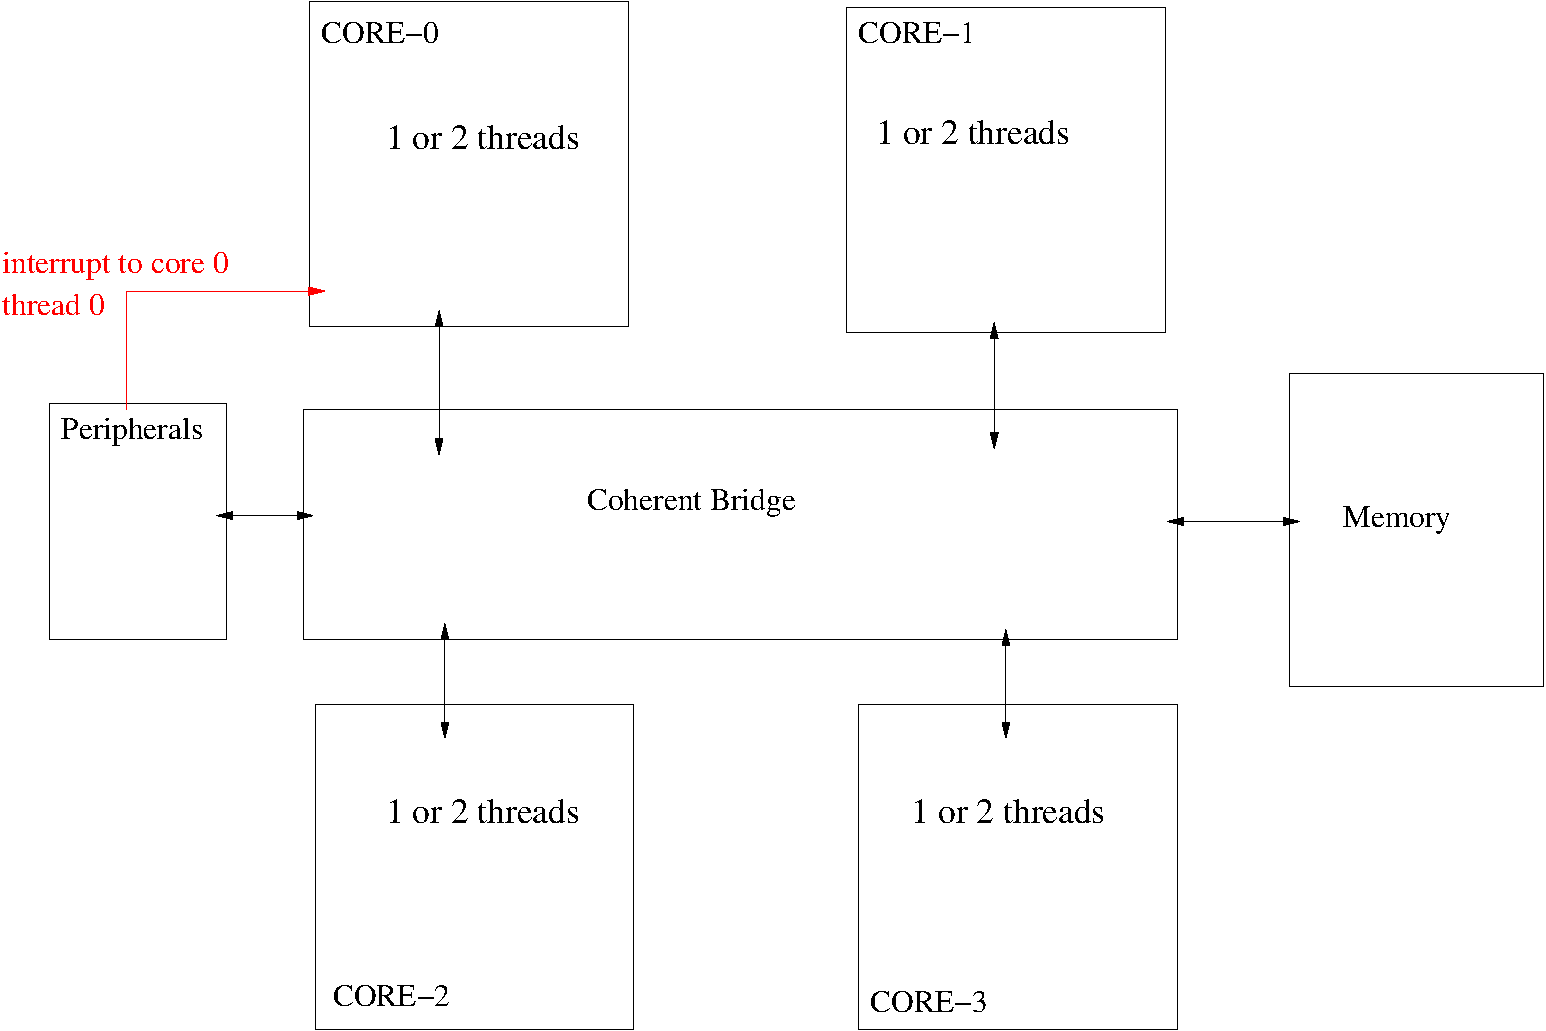
\includegraphics[width=10cm]{figs/MultiCore.pdf}
  \caption{AJIT Multi-core Processor System}
  \label{fig:MultiCore}
\end{figure}


}

\frame[containsverbatim]{\frametitle{AJIT core}

\begin{figure}
  \centering
  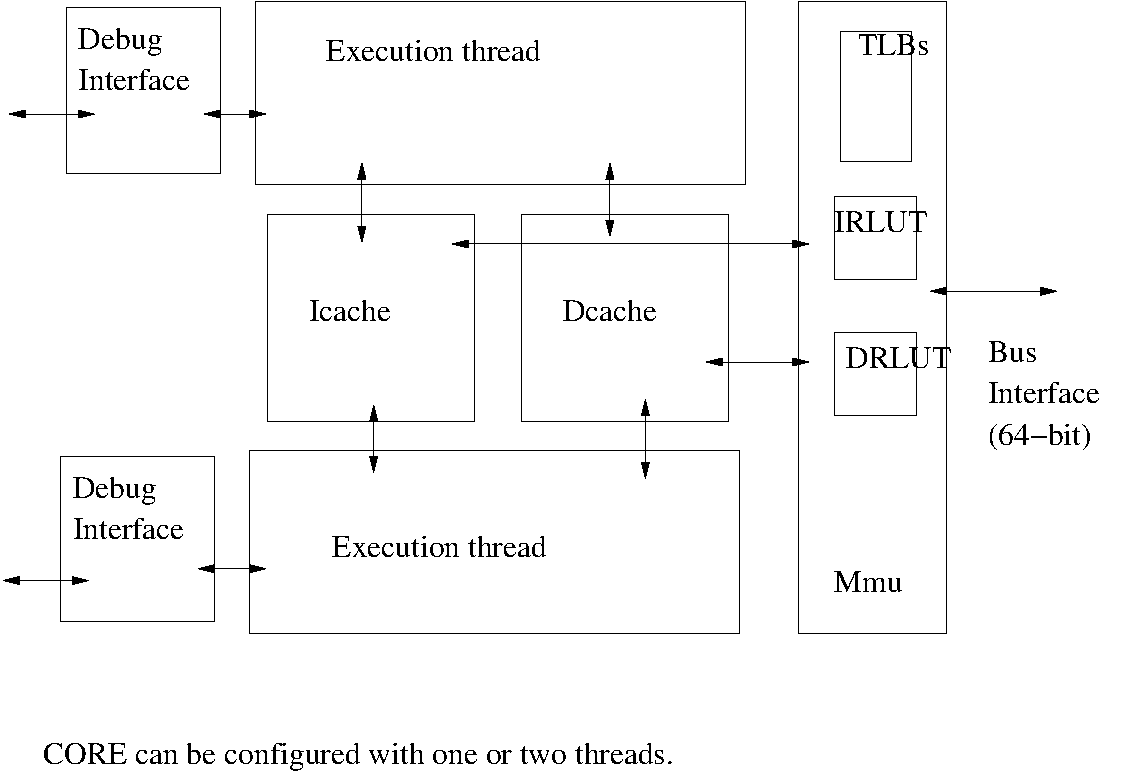
\includegraphics[width=10cm]{figs/CoreModel.pdf}
  \caption{AJIT Core with two threads}
  \label{fig:Core}
\end{figure}


}


\frame[containsverbatim]{\frametitle{Core and thread identification etc.}

\begin{itemize}
\item In each thread, a read of asr29 gives you the following 
word
\begin{verbatim}
 31:16          15:8        7:0
 0x5052         core-id     thread-id
\end{verbatim}
For instance, if you are in core 2, thread 1, then the read from
asr29 will return 0x50520201.
\item Note: two threads in the same core will share the caches
and the MMU.   This should be exploited by software.
\item Note: two threads in two different cores use distinct
caches and MMU.  In principle they can be executing distinct
processes with distinct virtual to physical address mappings.
\end{itemize}

}


\frame[containsverbatim]{\frametitle{System simulator}
\begin{verbatim}
ajit_C_system_model    ...options...
 
Important options:
     -n <number-of-cores>
     -t <number of threads per core>
     -u <32/64>   (ISA version: default is 32)
     -m <memory-map-file>  (Initial contents of RAM)

     [-w  <execution_trace_log_file>]
     [-d]  for post-condition checks
     [-r]  results file.
     [-l]  post-condition check log. 

 ... lots more ....
\end{verbatim}
}

\frame[containsverbatim]{\frametitle{Writing an application for bare-metal}

\begin{itemize}
\item Initialize the run time environment
\begin{itemize}
\item Set up stack for each thread.
\item Set up virtual->physical mapping for each thread.
\item Initialize processor state register, trap base register.
\end{itemize}
\item User program: as usual, but can use the following resources
\begin{verbatim}
AjitPublicResources/tools/ajit_access_routines
AjitPublicResources/tools/minimal_printf_timer
\end{verbatim}
\item Run compile script.  This will generate and ELF file, a memory map file and an object dump
file.
\item Run the program on the system simulator.
\end{itemize}

}

\frame[containsverbatim]{\frametitle{Walk through}
\begin{itemize}
\item Clone, and build.
\item Examine a test application.
\begin{itemize}
\item Initialization.
\item Compilation.
\item Run on the system model.
\item Examine results.
\end{itemize}
\end{itemize}
}


\end{document}
